\documentclass[a4paper, 11pt]{article}
%\usepackage[english]{babel}
\usepackage[dutch]{babel}
\usepackage{url}
\usepackage{listings}
\usepackage{a4wide}
\usepackage{booktabs}
\usepackage{parskip}
\usepackage{graphicx}

%handy commands
\newcommand{\tab}{\hspace*{2em}}
\newcommand{\tc} [1] {\textsc{#1}}

\title{Software Engineering en Gedistribueerde Applicaties \\ Werkplan}

\author{Victor Azizi \\ \url{azizivictor@gmail.com} \\ 6277861 \and
Arjen Tamerus \\ \url{arjen.tamerus@student.uva.nl} \\ 6330002 \and
Cedric Blom \\ \url{cedricblom@live.nl} \\ 6345107 \and
Timothy Dieduksman \\ \url{tgdieduksman@gmail.com} \\ 5935482 \and
Thomas Schoegje \\ \url{Thomas.Schoegje@student.uva.nl} \\10068767}

\begin{document}

\maketitle
%table of contents is not really needed here
%\tableofcontents
\clearpage

\section*{Introductie}
  In het project Software Engineering en Gedistribueerde Applicaties ontwikkelen wij op projectmatige manier een 
  opgave uit om zo praktische ervaring op te doen en groepsmatig te leren werken. Dit omvat onder andere het zelf
  bedenken en uitwerken van een implementatie volgens een werkplan dat we onderling hebben opgesteld, waarbij onder
  meer oefening in het werken met git weer aan de orde wordt gesteld. In dit werkplan bespreken we de opgave van de
  cli\"ent, de te behalen specificaties van het eindproduct, ons functionele ontwerp gevolgd door enkele specifieke
  implementatiekeuzes waarna we tenslotte de tijdsindeling presenteren en een korte toelichting geven aan de opdracht.

\section*{De opgave}
  De opgave die is ons voorgelegd is een gesimuleerde robot te programmeren om USAR (Urban Search And Rescue)
  operaties uit te kunnen voeren. Deze robot moet op zichzelf in zijn gesimuleerde omgeving kunnen rondrijden 
  zonder vast te lopen of te botsen, deze kunnen verkennen en in kaart brengen en tenslotte moet hij naar een 
  bepaald aangegeven punt kunnen rijden. De robot wordt dankzij het programma USARSim gesimuleerd op
  Windows XP computers met behulp van de Unreal Engine 2.5 
  (deze wordt bijgeleverd bij het spel Unreal Tournament 2004), en het programma behoort op afstand 
  aanstuurbaar te zijn via linux.

\section*{Doelstellingen}
  Gebaseerd op de wensen van de opdrachtgever zijn we tot de volgende specificaties gekomen waaraan we ons 
  eindproduct zullen laten voldoen:
  \begin{itemize}
   \item De robot moet kunnen rondrijden zonder te botsen of vast te lopen
   \item Hij moet de omgeving in kaart kunnen brengen
   \item Hij moet een pad kunnen plannen naar een bepaald aangegeven punt
   \item (Indien er afdoende tijd ter beschikking staat:) Hij moet bepaalde objecten (slachtoffers) kunnen herkennen
   \item Met behulp van tunnelling op afstand bestuurbaar
   \item Met een simpele interface en documentatie voor gebruiksvriendelijkheid
  \end{itemize}

\clearpage
\section*{Functioneel ontwerp}
  \begin{figure}[h!]
    \centering
      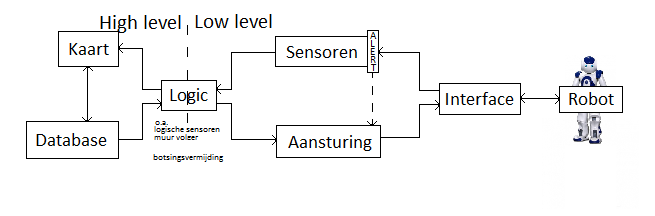
\includegraphics[scale=1]{eenplaatjemetheelduidelijkeuitleg.png}
    \caption{Het functionele ontwerp van onze implementatie.}
  \end{figure}

  We hebben besloten het probleem aan te pakken zoals te zien is in Figuur 1: tussen de robot en de rest van het
  systeem hebben we eerst een abstractielaag ingebouwd waarmee op bekende manier wordt gecommuniceerd door de rest
  van het systeem. Wanneer we een andere, vergelijkbare robot willen gebruiken waarmee op iets andere manier 
  gecommuniceerd moet worden kunnen we deze laag eenvoudig vervangen om de rest van het systeem te kunnen
  hergebruiken. Vanuit deze interface-laag wordt de informatie van de sensoren verstuurd naar een module die dit
  interpreteerd. Indien deze module merkt dat vlak voor de robot zich een object bevindt dan moet de robot 
  verteld worden te stoppen met bewegen, om zo een botsing te vermijden (dit gebeurt via een soort interrupt langs
  de Aansturingsmodule). Gewoonlijk wordt de sensor-informatie verstuurd naar de 'logica-module': dit is een
  verzamelnaam voor enkele hoger modules die iets doen met de ge\"interpreteerde informatie. Een deel van deze
  functionaliteit vindt plaats op een hoger, deliberatiever niveau (zoals de padplanner) terwijl er ook functies zijn
  die zich op reflexiever niveau afspelen (zoals de muurvolger). Vervolgens wordt sensorinformatie doorgespeeld
  naar een module verantwoordelijk voor het opbouwen van de kaart in de database, die vervolgens weer gebruikt
  wordt in de logica-module. Met behulp van deze informatie (maar ook op reflexiever niveau, direct met behulp van 
  informatie vanuit de sensoren) kan de logica-module hoger-niveau beslissingen nemen en hierop handelen door
  opdrachten naar de aansturing te versturen. Tenslotte stuurt de aansturing deze langs de 'vertaling' van de 
  Interface-laag naar de robot om deze zo te laten reageren op zijn opgeving.
  

\section*{Implementatiekeuzes}
  De omgeving zullen we in kaart brengen als een twee-dimensionaal grid waar de cellen verschillende waarden kunnen
  hebben voor begaanbaar terrein of verschillende soorten oppervlakten. We kunnen ons limiteren tot een twee-
  dimensionaal grid omdat de omgevingen waarin de robot zich zal bevinden platte bodems hebben: de oranje- en rode
  arena's zijn niet beschikbaar gesteld. Wanneer de robot toch merkt dat er sprake is van een hoogteverschil zoals
  bij een enkele helling in de gele arena zal hij dit markeren als ontoegankelijk en teruggaan naar waar hij 
  vandaan kwam. Let op dat hij zich niet enkel in de cellen kan bewegen, maar dat hij de kaart wel zo onthoudt.

  We voor Python gekozen als programmeertaal omdat we hierin efficient kunnen werken terwijl we dankzij de
  klassen ook makkelijk aan verschillende modulen tegelijk kunnen werken. Het is een
  hoog-niveau taal maar omdat er in onze implementatie geen sprake is van grootschalige data-verwerking of 
  opdrachten die een snelle verwerkingstijd vereisen. Tenslotte zal het verwerken van de informatie alsnog sneller
  gaan dan het verzenden van de opdrachten naar de robot, en is een vertraging daarom sowieso onvermijdbaar.

  Verder werken we tijdens het project met verscheidene systemen om de tijd die we aan productief werk besteden
  te kunnen verhogen. Hieronder vallen onder meer het revisie-controlesysteem Git om de code te delen en Google
  documents om gemakkelijk aantekeningen over beslissingen te maken en delen.


  
  Tenslotte hebben we ervoor gekozen tegelijkertijd met het ontwikkelen van de daadwerkelijke modules ook iemand
  te laten werken aan test-modules die gebruikt kunnen worden om te testen of de te gebruiken modules volledig
  werken zoals verwacht. Het specificeren van hoe een module getest wordt helpt bij het nadenken over wat fout
  kan gaan en om na te gaan of de module inderdaad zo werkt als andere modules zullen verwachten dat hij werkt.
  Het is natuurlijk ook een stuk makkelijker om uitgebreid een losse module te kunnen testen dan het moeten testen
  van complexere systemen van meerdere modules die samen tot onverwacht gedrag kunnen leiden. We kunnen bij het
  testen bijvoorbeeld GPS waarden gebruiken als ground truth om te kijken hoe nauwkeurig we de positie van onze
  robot weergeven.

\section*{Werkplan}
  \subsection*{Week 1}
    Doelstellingen:
    \begin{itemize}
        \item Inlezen en beginnen met project
	\item Werkende en geteste module voor het direct interpreteren van de sensoren.
	\item Werkende en geteste module voor het direct aansturen van de robot
	\item Functioneel skelet van het programma: kan de modules aansturen
	\item Interface-laag naar de robot
	\item Schets werkplan maken en bespreken met cli\"ent
	\item Opstelling eigen bibliotheek indien nodig
    \end{itemize}
    Werkverdeling:
    \begin{itemize}
        \item Skelet programma - \emph{Victor}
        \item Interpreteren sensoren - \emph{Arjen}
        \item Aansturen robot - \emph{C\'edric en Thomas}
        \item Testmodules - \emph{Timothy}
        \item Verslaggeving - \emph{Thomas}
    \end{itemize}
    
  \subsection*{Week 2}
    Doelstellingen:
    \begin{itemize}
	\item Definitieve werkplan maken en bespreken met cli\"ent
        \item Deliverable 1 afronden:
          \begin{itemize}
           \item Het grid dat hij gebruikt bij het bewegen moet aanwezig zijn (hoeft nog geen kaart te bouwen)
           \item Met behulp van dit grid kunnen rijden
           \item Botsingen voorkomen
          \end{itemize}
    \end{itemize}
    Werkverdeling:
    \begin{itemize}
        \item Afronden werkplan - \emph{Thomas}
        \item  \emph{TBA}
    \end{itemize}
    
  \subsection*{Week 3}
    Doelstellingen:
    \begin{itemize}
        \item Deliverable 1 demonstreren aan cli\"ent
        \item Inhoud Eindverslag en -experiment maken en bespreken met cl\"ent
        \item Draft verslag maken
    \end{itemize}
    Werkverdeling:
    \begin{itemize}
        \item \emph{TBA}
    \end{itemize}

  \subsection*{Week 4}
    Doelstellingen:
    \begin{itemize}
        \item Draft verslag bespreken met cli\"ent
        \item Eindpresentatie aan cli\"ent
        \item Eind-demonstratie aan cli\"ent
        \item Afronden en inleveren project (deliverable 2, urenverantwoording, code)
    \end{itemize}
    Werkverdeling:
    \begin{itemize}
        \item \emph{TBA}
    \end{itemize}
    
\section*{Discussie opgave}
  Al met al is het een interessante oefening vanaf grond af aan in groepsverband projectmatig te kunnen werken en
  is het een goede oefening voor het werken in de praktijk. Onze aanpak is duidelijk en we kunnen allen goed op weg
  om onze cli\"ent een bevredigend product af te leveren.

\end{document}
